\documentclass{oci}
\usepackage[utf8]{inputenc}
\usepackage{lipsum}
\usepackage{tikz}
\usetikzlibrary{shapes}

\title{Plataformas}

\begin{document}
\begin{problemDescription}
Ociman está a cargo del centro de operaciones de la OCI, donde se coordina la
final de la competencia y se revisan los problemas.
Para llegar a su destino sin ser visto, Ociman ha decidido usar un pogo stick,
saltando de edificio en edificio.

Vista desde arriba, la ciudad puede describirse como una grilla de $N\times N$
edificios.
Las filas y columnas son numeradas de norte a sur y de oeste a este con números
entre 1 y $N$.
Muchos de los edificios tienen techos irregulares y por lo tanto Ociman no
puede saltar sobre ellos.
Adicionalmente, Ociman tiene un límite de distancia para sus saltos y cada vez
que salta solo puede moverse a lo más $d$ edificios tanto horizontal como
verticalmente.

La siguiente imagen muestra un ejemplo para $N=6$ y $d=2$.
Los edificios sobre los cual Ociman \textbf{no} puede saltar están marcados con
una cruz.
Ociman está representado con un círculo y se encuentra en la coordenada $(3, 5)$.
El cuadrado en gris representa el área que Ociman puede alcanzar en un salto
estando en esa posición.
Dentro de ese área Ociman puede saltar a cualquier edificio que no está marcado
con una cruz.

\begin{center}
  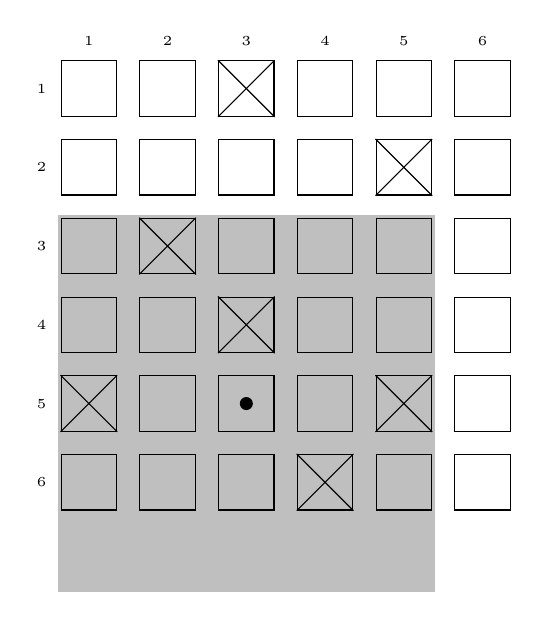
\begin{tikzpicture}[square/.style={regular polygon,regular polygon sides=4}]
    \draw [fill, lightgray] (-0.39, -1.39) rectangle +(4.78, 4.78);
    \foreach \i in {0,...,5} {
      \foreach \j in {0,...,5} {
        \node at (\i, \j) [rectangle, draw, scale=3] {};
      }
    }
    \foreach \i in {1,...,6} {
      \node at(\i-1, 5.6) {\tiny\i};
      \node at(-0.6, 6-\i) {\tiny\i};
    }
    \foreach \p in {(0,1), (2, 2), (4, 1), (4, 4), (3, 0), (1, 3), (2, 5)} {
      \node [cross out, draw, scale=2.9] at \p {};
    }
    \node [circle, fill, scale=0.5] at (2, 1) {};
  \end{tikzpicture}
\end{center}

Inicialmente Ociman comienza en el edificio en las coordenadas $(U, V)$ y tiene
que llegar al edificio en las coordenadas $(X, Y)$.
¿Podrá Ociman llegar al edificio de la OCI o deberá buscar otro plan?
En caso de ser posible, ?`cuál es el número mínimo de saltos que debe realizar
para llegar? 
\end{problemDescription}

\begin{inputDescription}
La primera línea de la entrada contiene dos enteros $N$ y $d$, que corresponden
respectivamente a las dimensiones de la ciudad ($1 < N$) y la distancia máxima
que puede saltar Ociman ($1 \le d < N$).

La segunda línea contiene dos enteros $U$ y $V$, que corresponden a las
coordenadas de la posición inicial de Ociman ($1 \le U, V \le N$).

La tercera línea contiene dos enteros $X$ e $Y$, que corresponden a las
coordenadas del edificio de la OCI ($1 \le X, Y \le N$).

Las siguientes $N$ líneas describen la ciudad.
Cada una de ellas contiene $N$ enteros.
El $i$-ésimo entero en la línea $j$-ésima contendrá un 1 si Ociman puede saltar
sobre el edificio en las coordenadas $(i, j)$ o 0 en caso contrario.
Se garantiza que tanto las coordenadas de la posición inicial de Ociman y las
coordenadas del edificio de la OCI tendrán edificios sobre los cuales se
puede saltar.
\end{inputDescription}

\begin{outputDescription}
Si Ociman puede llegar al edificio de la OCI, la entrada debe consistir
en un entero correspondiente al mínimo número de saltos que debe realizar para
lograrlo.
En caso contrario, la salida debe contener la palabra \verb-Inalcanzable-.
\end{outputDescription}

\begin{scoreDescription}
  % TBD distribución de puntajes
  \score{10} $1 \le N \le ?$. $B_{i,j}$ es siempre 1.
  \score{10} $1 \le N \le ?$. No hay restricciones adicionales.
\end{scoreDescription}

\begin{sampleDescription}
\sampleIO{sample-1}
\sampleIO{sample-2}
\end{sampleDescription}

\end{document}
